\documentclass{homework}
\author{Tomás Pérez}
\class{Mathematical Biostatistics Boot Camp 1}
\date{\today}
\title{Homework Assignments and Quizzes}

\graphicspath{{./media/}}

\begin{document} \maketitle

\section{Homework 1 - Week 1}
\begin{tcolorbox}[title=Question 1]
In a  random sample of 100 patients at a clinic, you would like to test whether the mean RDI is 10 or more using a one sided 5\% type 1 error rate.

The sample mean RDI was 12 with a standard deviation of 4. Do you reject the null hypothesis?
\end{tcolorbox}

Here we have a one sided test for a type I error rate of $\alpha = .05$. Our null hypothesis is $H_0: \mu = \mu_0 = 10$, where our sample size is made up of 100 patients, a sample mean RDI was $12$ with a standard deviation of $4$. Our test statistic is $TS = \frac{\bar{X}-\mu_0}{S/\sqrt{n}}$, and the alternative hypothesis is $H_a : \mu > \mu_0 = 10$ for example. We'll reject in favour of the alternative hypothesis if $TS \geq z_{1-\alpha}$, where $z_{1-\alpha}$ is the $(1-\alpha)$th standard normal quantile. Then, we can compute this with the following R routine

\begin{lstlisting}[language=R]
n <- 100
mu <- 12
mu0 <- 10 
sd <- 4
alpha <- .05

testStat <- (mu - mu0)/(sd/sqrt(n))
qtile <- qnorm(alpha, lower.tail = FALSE)

## We reject the null hypothesis if the test statistic is greater or equal than the quantile
reject <- testStat > qtile 
print(reject)

In [1]: TRUE
\end{lstlisting}

Then, we reject the null hypothesis in favour of the alternative hypothesis. \\

\begin{tcolorbox}[title=Question 2]
A pharmaceutical company is interested in testing a potential blood pressure lowering medication. Their first examination considers only subjects that received the medication at baseline then two weeks later. The data are as follows (SBP in mmHg)
\end{tcolorbox}

We are dealing with a pair of two non-independent data groups, thus we are to perform a two-sided paired test. Let $H_0: \mu_d = 0$ versus $H_a: \mu_d \neq 0$ where $\mu_d$ is the mean difference between followup and baseline. Our statistic of interest for this \textbf{ordinary paired two-group T-test} is 

$$
\frac{\bar{X}_d - \mu_{d0}}{S_d/\sqrt{n}}.
$$

Then, with the following R routine, we can know weather to reject or fail to reject the null hypothesis.

\begin{figure}
    \centering
    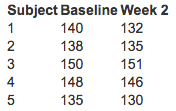
\includegraphics[scale=0.7]{figs/data points_week1.png}
    \caption{Data Points in mmHg}
    \label{fig:data}
\end{figure}

\begin{lstlisting}[language=R]
group1 = c(140,138,150,148,135) # R-array of group 1-data points
group2 = c(132,135,151,146,130) # R-array of group 2-data points
diff <- group2-group1 # difference of the two data groups
n <- sum(!is.na(diff)) # number of pairs of data points
mu <- mean(diff) # mean of the difference of the data groups
standard_deviation <- sd(diff) # standard deviation of the data groups 
testStat <- sqrt(n) * (mean(diff) - 0)/sd(diff) 

Pvalue <- 2 * pt(abs(testStat), n-1, lower.tail = FALSE) 
Pvalue

In [1]: 0.08652278
------------

group1 = c(140,138,150,148,135) # R-array of group 1-data points
group2 = c(132,135,151,146,130) # R-array of group 2-data points
t.test(group2, group1, alternative="two.sided", paired=TRUE)
t.test(diff)

Paired t-test

In [1]: data:  group2 and group1
In [2]: t = -2.2616, df = 4, p-value = 0.08652
In [3]: alternative hypothesis: true difference in means is not equal to 0
In [4]: 95 percent confidence interval:
In [5]: -7.5739122  0.7739122
In [6]: sample estimates:
In [7]: mean of the differences 
In [8]:             -3.4 
\end{lstlisting}

Note the equivalence with a two-sided paired T-test for a single data group

\begin{lstlisting}[language=R]
group1 = c(140,138,150,148,135) # R-array of group 1-data points
group2 = c(132,135,151,146,130) # R-array of group 2-data points
t.test(group2 - group1, alternative = "two.sided")

Paired t-test

In [1]: data:  group2 and group1
In [2]: t = -2.2616, df = 4, p-value = 0.08652
In [3]: alternative hypothesis: true difference in means is not equal to 0
In [4]: 95 percent confidence interval:
In [5]: -7.5739122  0.7739122
In [6]: sample estimates:
In [7]: mean of the differences 
In [8]:             -3.4 
\end{lstlisting}

But this is not equivalent to a one-sided two-sided test:

\begin{lstlisting}[language=R]
group1 = c(140,138,150,148,135) # R-array of group 1-data points
group2 = c(132,135,151,146,130) # R-array of group 2-data points

In [1]: Paired t-test
data: group2 and group1
In [2]: t = -2.262, df = 4, In In [3]: p-value = 0.04326
In [3]: alternative hypothesis: In [4]: true difference in means is less than 0
In [5]: 95 percent confidence interval:
In [6]: -Inf -0.1951
In [7]: sample estimates:
In [8]: mean of the differences
In [9]:             -3.4
\end{lstlisting}

In conclusion, the P-value is equal to .09 and we fail to reject the null hypothesis. \\ 

\begin{tcolorbox}[title=Question 3]
A sample of 9 men yielded a sample average brain volume of 1,100cc and a standard deviation of 30cc. For what values of $\mu_0$ would a test of $H_0: \mu = \mu_0$  fail to reject the null hypothesis in a two sided 5\% Students t-test?
\end{tcolorbox}

Here we just need to construct the 95\% Student's $T$ confidence interval.

\begin{lstlisting}[language=R]
n <- 9
mu0 <- 1100
sd <- 30

CI <- (c(-1,1) * qt(0.975,n-1) * sd/sqrt(n-1) + mu0)
CI

In [1]: 1075.541 1124.459
\end{lstlisting}

Thus, we find the answer is $[1076cc, 1124 cc]$. \\

\begin{tcolorbox}[title=Question 4]
To further test a hospital triage system, administrators selected 200 nights and randomly assigned a new triage system to be used on 100 nights and a standard system on the remaining 100 nights. They calculated the nightly median waiting time (MWT) to see a physician. The average MWT for the new system was 4 hours with a standard deviation of .5 hours while the average MWT for the old system was 6 hours with a standard deviation of 2 hours. Test the hypothesis of a decrease in the mean MWT associated with the new treatment using a two sided 5\% Z test. Does it appear to be effective?
\end{tcolorbox}

Let $H_0: \mu = 0$ be the null hypothesis (ie. there's no difference in response times between the hospital triage systems). In this case, we have to construct a 95\% Student's $T$-test for the difference of two random variables. Assuming our data are iid Gaussian and given that $n_1, n_2 \gg 1$ we can use the standard normal quantiles, then the statistic of interest is 

$$
\bar{Y}-\bar{X}\pm z_{1-\frac{\alpha}{2}} \sqrt{\frac{S_x^2}{n_X}+\frac{S_y^2}{n_Y}}.
$$

\begin{lstlisting}[language=R]
n_old <- n_new <- n_pairs <- 100
mu_old <- 4
sd_old <- .5 
n_new <- 100
mu_new <- 6
sd_new <- 2
test_stat <- mu_new - mu_old + c(-1, 1) * qnorm(0.975) * sqrt(sd_new^2/n_new + sd_old^2/n_old)
test_stat

In [1]: 1.595943 2.404057
\end{lstlisting}

Since this interval doesn't contain zero, we reject the null hypothesis and conclude that the new system does reduce MWTs. \\

\begin{tcolorbox}[title=Question 5]
Suppose that 18 obese subjects were randomized, 9 each, to a new diet pill and a placebo. Subjects’ body mass indices (BMIs) were measured at a baseline and again after having received the treatment or placebo for four weeks. The average difference from follow-up to the baseline (followup - baseline) was -3 kg/m2 for the treated group and 1 kg/m2 for the placebo group. The corresponding standard deviations of the differences was 1.5 kg/m2 for the treatment group and 1.8 kg/m2 for the placebo group. Does the change in BMI over the two year period appear to differ between the treated and placebo groups?  Assuming normality of the underlying data and a common population variance, give the relevant 95\% t confidence interval.
\end{tcolorbox}

\begin{lstlisting}[language=R]
n <- 9
mu_treated <- -3
sd_treated <- 1.5

mu_placebo <- 1
sd_placebo <- 1.8

Sp <- sqrt((n-1)/(n+n-2)*sd_treated + (1-(n-1)/(n+n-2))*sd_placebo)

(mu_treated - mu_placebo)/(Sp*sqrt(1/n + 1/n))
\end{lstlisting}

\begin{tcolorbox}[title=Question 6]
Suppose that 18 obese subjects were randomized, 9 each, to a new diet pill and a placebo. Subjects’ body mass indices (BMIs) were measured at a baseline and again after having received the treatment or placebo for four weeks. The average difference from follow-up to the baseline (followup - baseline) was -3 kg/m2 for the treated group and 1 kg/m2 for the placebo group. The corresponding standard deviations of the differences was 1.5 kg/m2 for the treatment group and 1.8 kg/m2 for the placebo group. Does the change in BMI over the two year period appear to differ between the treated and placebo groups?  Assuming normality of the underlying data and a common population variance, give the relevant 95\% t confidence interval.
\end{tcolorbox}

\begin{lstlisting}[language=R]
n <- 9
mu_treated <- -3
sd_treated <- 1.5

mu_placebo <- 1
sd_placebo <- 1.8

Sp <- sqrt((n-1)/(n+n-2)*sd_treated + (1-(n-1)/(n+n-2))*sd_placebo)

CI <- (mu_treated-mu_placebo) + c(-1,1)*(qt(.975, 9+9-2) * Sp * sqrt(2/n))
CI
\end{lstlisting}

\begin{tcolorbox}[title=Question 7]
Suppose that systolic blood pressures were taken on 16 oral contraceptive users and 16 controls at baseline and again then two years later. The average difference from follow-up SBP to the baseline (followup - baseline) was 11 mmHg for oral contraceptive users and 4 mmHg for controls. The corresponding standard deviations of the differences was 20 mmHg for OC users and 28 mmHg for controls. Assuming that blood pressure are normally distributed and an equal variance, give a P-value for a two sided hypothesis test that the change in BP differs for OC users compared to controls.
\end{tcolorbox}

\begin{tcolorbox}[title=Question 8]
Researchers would like to conduct a study of 100 healthy adults to detect a four year mean brain volume loss of $.01~mm^3$. Assume that the standard deviation of four year volume loss in this population is $.04~mm^3$. What would be the power of the study for a 5\% one sided test versus a null hypothesis of no volume loss?
\end{tcolorbox}

\begin{tcolorbox}[title=Question 9]
The Daily Planet ran a recent story about Kryptonite poisoning in the water supply after a recent event in Metropolis. Their usual field reporter, Clark Kent, called in sick and so Lois Lane reported the stories. Researchers sampled 288 individuals and found mean blood Kryptonite levels of 44, both measured in Lex Luthors per milliliter (LL/ml). They compared this to 288 sampled individuals from Gotham city who had an average level of 42.04. Report the Pvalue for a two sided Z test of the relevant hypothesis. Assume that the standard deviation is 12 for both groups.T
\end{tcolorbox}

\begin{tcolorbox}[title=Question 10]
As your variance goes up, what happens to power?
\end{tcolorbox}

\begin{tcolorbox}[title=Question 11]
Suppose that you have three independent samples from a $N(\mu_1, \sigma^2)$, $N(\mu_2, \sigma^2)N$ and $N(\mu_3, \sigma^2)$ respectively of size $n_1$, $n_2$ and $n_3$. Let $S_1^2$, $S_2^2$ and $S_3^2$ be the associated sample variances. Would $\frac{1}{3}S_1^2 + \frac{1}{3} S_2^2 + \frac{1}{3} S_3^2$ be unbiased?
\end{tcolorbox}

\begin{tcolorbox}[title=Question 12]
Consider any of the hypothesis tests we've covered in class. If you know you reject at a specific level of $\alpha$, then you know what else?
\end{tcolorbox}

\begin{tcolorbox}[title=Question 13]
Consider a one sided $\alpha$ level single group Z test of $H_0 : \mu = \mu_0$ versus the alternative $H_a : \mu < \mu_0$ with the data $\bar X$ for the sample mean and s for the sample standard deviation with n measurements. What are the collection of points for which you would fail to reject the hypothesis?
\end{tcolorbox}

\clearpage

\section{Quiz 1 - Week 1}

\begin{tcolorbox}[title=Question 1]
\end{tcolorbox}

\clearpage

\section{Homework 2 - Week 2}

\begin{tcolorbox}[title=Question 1]
\end{tcolorbox}

\clearpage

\end{document}
